\chapter*{Conclusion and perspectives}
\addstarredchapter{Conclusion}
\markboth{Conclusion}{Conclusion}
\label{sec:conclusion}

\section*{Conclusion}
By considering usual classifiers (\textit{e.g.}, $k$-NN) that are based on distance between samples, we have proposed a Multi-modal and Multi-scale Temporal Metric Learning (\textsc{m$^2$tml}) framework for a robust $k$-NN classifier. It is based on a new space representation, the pairwise dissimilarity space, where pairs of time series are embedded as vectors described by different basic temporal metrics. A metric combining the basic metrics can be seen as a function (linear or non-linear) of the pairwise dissimilarity space, learned by using a large margin optimization process (\textsc{svm}) inspired from the nearest neighbors metric learning framework. The obtained metric satisfies the properties of a dissimilarity (positivity, reflexivity, symmetry), leads to good performances on a large number of public datasets, and gives an interpretable solution that allows us to analyze the modalities and scales that are the most discriminant.

Temporal data may be compared based on various characteristics, called modalities. Time series can be compared not only on their amplitudes like static data, but also on other modalities such as their behavior, frequency, etc. To cope with delays in real time series, Dynamic time warping approach can be used to re-align the signals.  Some authors propose to combine several modalities through a combination function but the combinations are either, limited to two modalities or in the case of multiple modalities (more than 2), the number of parameters to optimize for a classifier may become time consuming. In general, state of the art approaches compared the time series by involving all observations, restricting the potential of comparison measures (metrics) to capture local differences. We proposed to take into account local characteristics, that we named multi-scale. We have believed that all of these considerations (modality, scale, delays) should be taken into consideration in the definition of a metric in order to improve the performance of the classifier.

The objective is to learn a metric for a robust $k$-NN. For that, we propose a general formalization of the problem of learning a combined multi-modal and multi-scale temporal metric (\textsc{m$^2$tml}). Based on a pairwise dissimilarity representation of the pairs of time series, the metric learning problem can be reduced to the learning of a linear or non linear function of the dissimilarity space that satisfies the properties of a dissimilarity. Inspired from metric learning work, the problem is formalized as an optimization problem involving a regularization and loss term which aims to pull samples that are expected to be similar and push away samples that should be dissimilar. First, by considering a linear combination of the basic metrics, changing the regularization term leads the general formalization to a linear and quadratic formalization. The latter allows us to extend to the learning of non-linear functions thanks to the "kernel" trick. However, the methods can lead to functions that doesn't meet the properties of a dissimilarity (non-positivity). Secondly, we propose to formulate the problem as a \textsc{svm} problem which aims to separate pull and push samples, then we define a metric that satisfies the required properties of a dissimilarity. 

The efficiency of the proposed \textsc{svm}-based solution has been tested in the case of classification of univariate time series, on a wide variety of datasets coming from various fields (simulated data, medicine, power consumption, etc.), diverse sizes of training and testing, various number of classes, etc. The \textsc{m$^2$tml} solution achieves not only, either equivalent or better performances compared to the standard global metrics (Euclidean distance, dynamic time warping, temporal correlation, Fourier-based distance), but it also provides a sparse and interpretable solution that allows us to give a comprehensive analysis of the most discriminative modalities and their respective temporal granularity that may not be always intuitive \textit{a priori}. 

\section*{Perspectives}
\subsection*{Extension to other modalities, multivariate problems and other type of data}
In this work, we only focus on three basic temporal metrics (euclidean distance, temporal correlation, Fourier-based distance). Montero \& Vilar propose in \cite{Montero2014} a review on a wide number of metrics dedicated to time series. For remaining challenging datasets in our experiments, it could be interesting to integrate other basic temporal metrics in our framework to see the obtained results.

\noindent The framework can be easily extend to multivariate problem. For each dimension, we consider the set of multi-modal and multi-scale description. Then,  we consider the union over the dimensions as the pairwise dissimilarity description $d_1, \ldots, d_p$. 

\noindent The proposed solution has been tested in the case of time series data but the framework is more general. It can be applied to any other type of data (strings, graphs, images) to learn a combined metric. These data might be compared on other characteristics. Deza \& Deza makes a detailed review of metrics for various domains in \cite{Deza2009}.


\subsection*{Other possibilities for the multi-scale description}
A second improvement is about the multi-scale description that denotes in this work as a temporal segmentation. We propose a multi-scale approach based on a binary segmentation using a dichotomy process. Other solutions could be proposed, in particular, in order to localize automatically finely events of interest. For example, in the case of the dataset SonyAIBO, the discriminative temporal locations of the signal is known \textit{a priori} (Fig. \ref{fig:SonyAIBO_tmp}). With the actual multi-scale description, it is not possible to extract exactly the two red patterns of interest. A solution based on a sliding window of variable lengths could be used to locate precisely these patterns. 

\begin{figure}[h!]
	\centering
	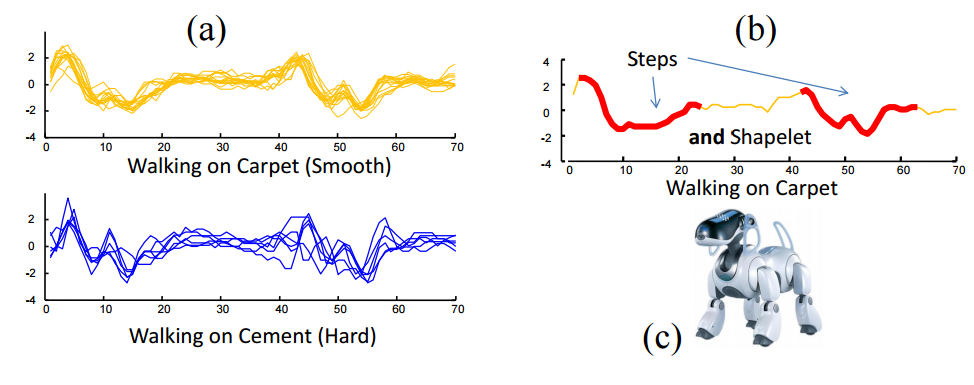
\includegraphics[width=1\linewidth]{SonyAIBO_temp}
	\caption{(a) Two classes of time series from the Sony AIBO accelerometer. (b) The and-shapelets from the walk cycle on carpet. (c) The Sony AIBO Robot.\protect\footnotemark}
	\label{fig:SonyAIBO_tmp}
\end{figure}
\footnotetext{source: \url{http://www.cs.ucr.edu/~eamonn/LogicalShapelet.pdf}}

\subsection*{Learning of local metrics}
Some authors suggest that in some datasets, global linear metric learning approach may not be sufficient to improve the accuracy of $k$-NN classification \cite{Weinberger2009, Wang2012}. Since the discriminatory power of the input features might vary between different neighborhoods, learning a global metric cannot fit well the distance over the data. To overcome this difficulty, they propose to learn a metric on each neighborhood, referred to as local metric learning. \\
Similarly, the \textsc{m$^2$tml} framework could be extended to learn local combined temporal metrics for each neighborhood. The objective is to learn for each $n$ set $Pull_i$ and $Push_i$ ($n$ being the number of samples in the training set) a local metric using the same framework than the one we propose in this work. We obtain $n$ local metrics $D_i$. Then, to classify a new sample $\textbf{x}_{test}$, we compute the $n$ metrics $D_i(\textbf{x}_{i,test})$ and classify $\textbf{x}_{test}$ using the $k$ lowest distances $D_i(\textbf{x}_{i,test})$.


\subsection*{Re-iteration of the initial metric}
Similarly to Large Margin Nearest Neighbors (\textsc{lmnn}) approach proposed by Weinberger \& Saul \cite{Weinberger2009}, the \textsc{m$^2$tml} approach might inherit the same problem of the initial distance, \textit{i.e.}, fixing the set $Pull_i$ and $Push_i$ according to an initial distance (Euclidean distance in this work). Other initial distances could have been used. If the initial distance is far away from the optimal solution, the definition of the sets $Pull_i$ and $Push_i$ can impact the convergence to the optimal solution. In same spirit as the multi-pass \textsc{lmnn} approach proposed by Weinberger \& Saul, we could re-iterate the learning process. At each step, we re-define the sets $Pull_i$ and $Push_i$ using the distance learned at the previous step. Then, we stop the learning when arriving at convergence (\textit{e.g.}, the sets $Pull_i$ and $Push_i$ doesn't evolve anymore or evolve slightly between two steps).

\subsection*{Other propositions to define the combined metric}
First, as said in Section \ref{sec:svm_based}, note that the framework to define the metric $D$ and $D_\mathcal{H}$ can also be used in the linear and quadratic formalization. However, the obtained solution for $D$ and $D_\mathcal{H}$ can be far away from the original form of $D$ that has been optimized in the optimization problem.

Secondly, we have proposed a form for the metric $D$ and $D_\mathcal{H}$ so that it satisfies the properties of a dissimilarity. Other solutions could have been proposed. In particular, instead of using a max operator in the definition of $D$ and $D_\mathcal{H}$, an other variant could consider a parameter $\lambda$ that can be either positive or negative. In the case of negative $\lambda$, the action of the exponential term would become a pull term instead of a push term. Note that in both cases, for extreme value of $\lambda$, there exists a risk to binarize the metric. In particular, for $\lambda \mapsto - \infty$, there exists a risk of having zero values for the nearest neighbors, which could lead to problems when classifying by the nearest neighbors. 

\subsection*{Extension to regression problems}
For the \textsc{svm}-based solution, in the pairwise dissimilarity space, each vector $\textbf{x}_{ij}$ is labeled $y_{ij}$ by following the rule: if $\textbf{x}_i$ and $\textbf{x}_j$ are similar, the vector $\textbf{x}_{ij}$ is labeled -1; and +1 otherwise. \\
For classification problems, the concept of similarity between samples $\textbf{x}_i$ and $\textbf{x}_j$ is driven by the class label $y_i$ and $y_j$ in the original space:
\begin{equation}
y_{ij} = 
\left\{
\begin{split}
+1 \text{\quad if } y_i = y_j\\ 
-1 \text{\quad if } y_i \neq y_j
\end{split}
\right.
\end{equation}
For regression problems, each sample $\textbf{x}_i$ is assigned to a continuous value $y_i$. Two approaches are possible to define the similarity concept. The first one discretizes the continuous space of values of the labels $y_i$ to create classes. One possible discretization bins the label $y_i$ into $Q$ intervals as illustrated in Fig. \ref{fig:Discretize_binning}. Each interval becomes a class which associated value can be set for example as the mean or median value of the interval. Then, the classification framework is used to define the pairwise label $y_{ij}$.

\begin{figure}[h!]
	\centering
	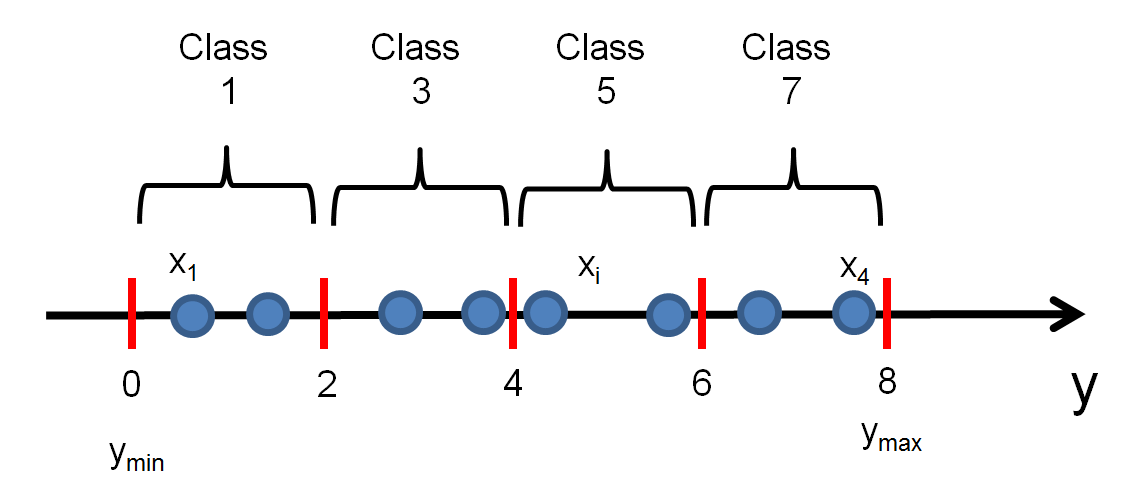
\includegraphics[width=0.5\linewidth]{images/Discretize_binning}
	\caption[Example of discretization by binning a continuous label $y$ into $Q=4$ equal-length intervals.]{Example of discretization by binning a continuous label $y$ into $Q=4$ equal-length intervals. Each interval is associated to a unique class label. In this example, the class label for each interval is equal to the mean in each interval.}
	\label{fig:Discretize_binning}
\end{figure}

\noindent This approach may leads to border effects between the classes. For instance, two samples $\textbf{x}_i$ and $\textbf{x}_j$ that are close to a frontier and that are on different sides of the border will be considered as different, as illustrated in Fig \ref{fig:Discretize_binning_border_effect}. Moreover, a new sample $\textbf{x}_j$ will have its labels $y_j$ assigned to a class and not a real continuous value. 

\begin{figure}[h!]
	\centering
	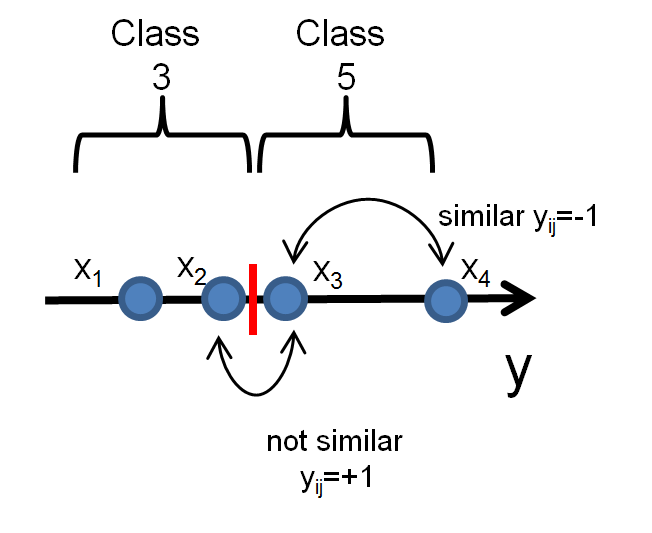
\includegraphics[width=0.35\linewidth]{images/Discretize_binning_border_effect}
	\caption[Border effect problems.]{Border effect problems. In this example, $\textbf{x}_2$ and $\textbf{x}_3$ have closer value labels $y_2$ and $y_3$ than $\textbf{x}_3$ and $\textbf{x}_4$. However, with the discretization $\textbf{x}_2$ and $\textbf{x}_3$ don't belong to the same class and thus are consider as not similar.}
	\label{fig:Discretize_binning_border_effect}
\end{figure}

\noindent The second approach considers the continuous value of $y_i$, computes a $L_1$-norm between the labels $|y_i-y_j|$ and compare this value to a threshold $\epsilon$. Geometrically, a tube of size $\epsilon$ around each value of $y_i$ is built. Two samples $\textbf{x}_i$ and  $\textbf{x}_j$ are considered as similar if the absolute difference between their labels $|y_i-y_j|$ is lower than $\epsilon$ (Fig. \ref{fig:pairwise_label_tube}):
\begin{equation}
y_{ij} = 
\left\{
\begin{split}
\begin{aligned}
-1 & \text{\quad if } |y_i-y_j| \leq \epsilon \\ 
+1 & \text{\quad otherwise }
\end{aligned} 
\end{split}
\right.
\end{equation}

\begin{figure}[h!]
	\centering
	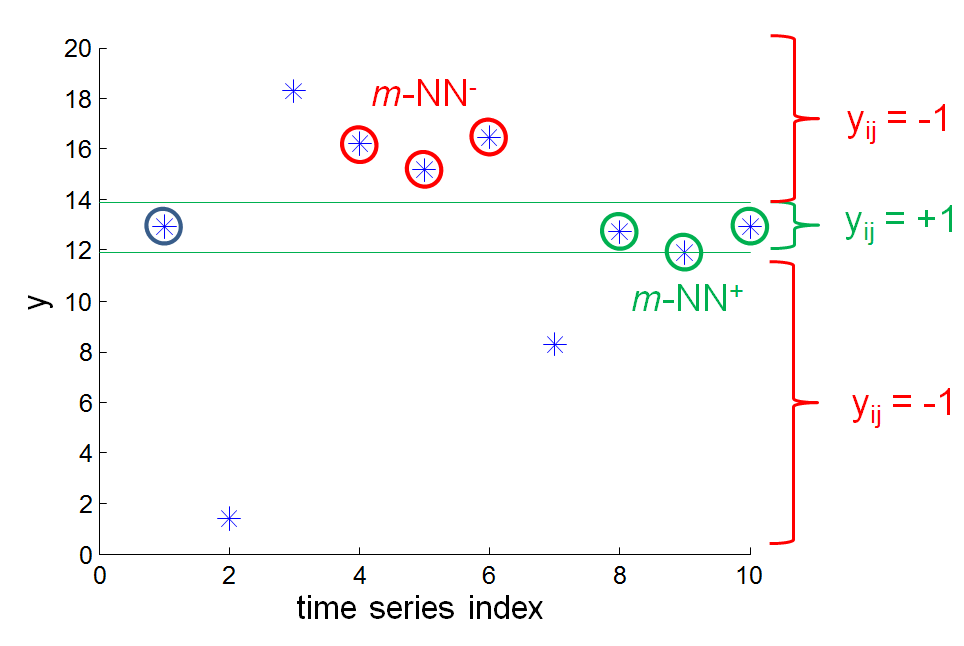
\includegraphics[width=0.55\linewidth]{images/pairwise_label_tube2}
	\caption[Example of pairwise label definition using an $\epsilon$-tube (green lines) around the time series $\textbf{x}_i$ (circled in blue).]{Example of pairwise label definition using an $\epsilon$-tube (green lines) around the time series $\textbf{x}_i$ (circled in blue). For, time series $\textbf{x}_j$ that falls into the tube, the pairwise label is $y_{ij} = -1$ (similar) and outside of the tube, $y_{ij} = +1$ (not similar). $m$-NN$^+$ and $m$-NN$^-$ time series are indicated respectively in green and red circle for $k$-NN with $k=1$ and $m=3$ neighborhood.}
	\label{fig:pairwise_label_tube}
\end{figure}


\subsection*{Using the learned combined metric in other algorithms}
In this work, we propose to learn a temporal metric for a robust $k$-NN classifier. As explained in Section \ref{sec:kNN}, for industrial practical usage, the $k$-NN algorithm may present some disadvantages, mainly due to its computational complexity, both in memory space (storage of the training samples) and time (search of the neighbors). \\
Inspired from the work on temporal trees in \cite{AhlameDouzal-Chouakria2012}, we could use the learned metric in an other classifier such as a decision tree. For multivariate classification problems, an idea could be to learn in a first step a linear or non-linear multi-modal and multi-scale temporal metric for each dimension. Then, in a second step, given the set of multi-modal and multi-scale temporal metrics, we build a temporal tree based on the training samples: First, for each dimension, we split the data into two partitions using a clustering algorithm such as $k$-means ($k=2$) with the learned temporal metric for the considered dimension. Secondly, similarly to classical decision tree, we compute a criterion (\textit{e.g.}, a Gini coefficient or Information Gain coefficient) to select the best split, \textit{i.e.}, the best learned temporal metric that minimize the criterion. Thirdly, we compute for each partition the centroid, \textit{i.e.}, the time series that minimizes the mean distance over all the other time series in the same partition. Then, for each obtained partition, we re-iterate the process until the stopping condition is met, \textit{e.g.}, all the sample in the partition have the same class label or the number of sample have fallen below some minimum threshold. It corresponds a leaf node and the label of the node is assigned to the one of the majority. To classify a new time series $\textbf{x}_{test}$, similarly to classical decision tree, at each node, we compute the distance $D$ or $D_\mathcal{H}$ of the new sample to each centroid. The time series $\textbf{x}_{test}$ is then assigned to the node of the nearest centroid until it reaches a leaf node where its label is assigned.



%\begin{itemize}
%%	\item Bilan des apports de la thèse.
%%		\begin{itemize}
%%			\item \textbf{Objectif}: Dans cette thèse, nous nous sommes intéressés à l'apprentissage de métriques combinées multi-modal et multi-échelle en vue d'une classification kNN robuste.
%%			\item \textbf{Uni-modal}: Les données temporelles, contrairement aux données statiques, peuvent être comparés non seulement sur la base de modalités comme les valeurs mais aussi au moins, sans être exhaustifs sur la base de modalités temporelles comme la forme ou la fréquence. De manière classique, la comparaison de séries se fait sur la base d'une modalité à l'échelle globale qui définit les mesures de distance habituellement utilisées (distance euclidienne, corrélation temporelle, distance à base Fourier, etc.).
%%			\item \textbf{Multi-modal}: Afin de tenir compte de plusieurs modalités au sein d'une même métrique, certains auteurs ont proposés de combinés plusieurs modalités via des fonctions de combinaisons. Elles sont en général limités à 2 modalités et sont définis sans considération du classifieur. La recherche des meilleurs paramètres peut devenir lourd computationnelement en augmentant le nombre de métriques impliqués dans la combinaison.
%%			\item \textbf{Multi-échelle}: Ce travail a mis en évidence l'importance de comparer les séries temporelles à différentes échelles temporelles. Les modalités et métriques cités précédemment peuvent être adaptées afin de comparer les séries, non seulement sur la base de l'échelle globale (impliquant l'ensemble des éléments de la série temporelle) mais aussi à une échelle plus localisées (impliquant une partie des éléments de la séries temporelles).
%%			\item \textbf{Metric Learning}: Afin d'améliorer les performances d'un classifieur kNN, certains travaux dans la littérature se sont intéressés à l'apprentissage de la métrique en vue d'une classification robuste kNN. Ces approches reposent en général sur l'apprentissage d'une distance de Mahalanobis dans un cadre linéaire ou non-linéaire. Certains parrallèles avec les SVM ont aussi été étudiés. Les travaux sont nombreux pour les données statiques, moins nombreux pour les données structurées, et en particulier encore dans ses début pour les séries temporelles.
%%			\item \textbf{Formalisation}: La seconde partie de ce travail a abouti à la formalisation du problème d'apprentissage métriques combinées multi-modal et multi-échelle en vue d'une classification kNN robuste.
%%			\item \textbf{Espace des paires}: Le calcul d'une métrique impliquant toujours deux éléments, nous avons proposé de représenter les paires de séries temporelles dans un espace de dissimilarités où chaque dimension est une métrique temporelle de base (i.e., une modalité à une échelle temporelle). L'apprentissage d'une métrique combinée de plusieurs métriques temporelle de base se ramène alors à l'apprentissage d'une fonction dans l'espace de dissimilarités qui vérifie au moins les propriétés d'une dissimilarité (positivité, reflexivité, symétrie). Rappelons que l'interprétation de proximité dans cet espace sur la proximité des séries dans l'espace d'origine doit être fait avec prudence.
%%			\item \textbf{m2tml optimisation}: le problème d'apprentissage de la métrique combinées peut être de manière général ramené à un problème d'apprentissage de métrique. Il est formalisé sous la forme d'un problème d'optimisation impliquant 3 termes: 1) un terme de régularisation dont le but est de rapprocher les paires pull (similaires). 2) un terme loss dont le but est d'éloigner les paires push (dissimilaires). 3) des contraintes liés aux paires dissimilaires. Plusieurs stratégies pour construire les ensembles pull et push ont été proposés. La solution retenue est celle des mNN+ vs mNN-. Nous pensons qu'en élargissant en apprentissage le voisinage au m plus proche permettra de mieux généraliser la métrique lors du test.
%%			\item \textbf{Les différentes formalisations}: Depuis le problème général, nous avons proposé 3 formalisations impliquant différentes régularisations ou frameworks: linéaire, quadratic, basé svm. Dans la formalisation linéaire, le terme de régularisation est linéaire et la métrique combinée est une combinaison linéaire des métriques de bases, vérifiant les propriétés d'une dissimilarité. Dans la formalisation quadratique, le terme de régularisation est quadratique. Similairement au développement svm, le problème peut être transformé sous une forme n'impliquant que des produits scalaires, permettant d'étendre l'apprentissage de la métrique combinée à des combinaisons à la fois linéaire comme non-linéaire via le kernel trick. La métrique apprise ne vérifie pas cependant les propriétés d'une dissimilarité (non-positive). 
%%			\item \textbf{Solution basée svm}: Dans le framework basé svm, la fonction de distance n'est pas connue a priori. Le but est de construire un classifieur svm qui permet de séparer les ensembles pull et push. Sur la base de la solution obtenue du classifieur, une métrique est bâtie qui respecte les propriétés d'une métrique. En particulier, on souligne 2 éléments importants impliqués dans la métrique: la norme du projeté, la distance à la marge du projeté. La norme du projeté d'une paire permet de mesurer la proximité entre les séries temporelles impliquées dans la paire, d'après les features retenus pour séparer les classes pull et push. Afin d'assurer que la norme des paires push soit inférieurs à celles des paires pull, la distance du projeté à la marge nous permet de déterminer l'appartenance d'une paire à l'ensemble pull ou push. Le terme push est donné par une transformation exponentielle de la distance à la marge du projeté contrôlé par un paramètre qui mesure la force du terme push en fonction de la configuration des données. Grâce au framework svm, la méthode peut être naturellement étendu pour apprendre des fonctions non-linéaires.
%%			\item \textbf{Pre-processing lié au svm}: La solution svm retenue nous amène à des éléments de pré-processing nécessaire: normalisation de l'espace des dissimilarités, normalisation des voisinages. 
%%			\item \textbf{Expérimentation}: L’efficacité de la méthode proposée m2tml a été vérifiée dans un vaste nombre de données publiques dans le cadre d'une classification 1NN de séries temporelles univariées. Les données considérées étaient de domaines divers, de nombres de classes divers, avec des tailles de séries courtes et longues et un nombre divers de séries en apprentissage. Certaines de ces bases obtiennent des scores concluant avec les métriques valeurs classiques (euclidienne, dtw) et d'autres sont encore ouverts à des améliorations. La méthode proposées m2tml permet d'obtenir soit des scores équivalents aux métriques classiques globales, soit d'améliorer les résultats de la classification. Comparativement aux combinaisons a priori, la méthode atteint des performances similaires mais permet d'ajouter des métriques sans devoir ajouter de nouveaux paramètres à optimiser. Soulignons l'avantage supplémentaire de la méthode à interpréter les résultats obtenus: elle permet de localiser les modalités et localisations temporelles d'intérêt par apprentissage qui permet de purifier les voisinages. Ainsi, lorsque dans le cadre d'une utilisation industrielle, en l'absence de connaissance a priori sur les séries, la méthode permet de comprendre ce qui permet de discriminer au mieux les séries afin d'avoir des voisinages purifiées.
%%		\end{itemize}
%	\item Perspectives
%	\begin{itemize}
%		\item \textbf{Extension à d'autres modalités}: Le travail effectué s'est intéressé à 3 types de distance (distance euclidienne, corrélation temporelle, distance à base Fourier). Il existe cependant d'autres mesures de distance pour les séries temporelles qu'il serait intéressant d'étudier (wavelets, MFCC, etc.) (cf article).
%		\item \textbf{Découpage multi-échelle}: Dans ce travail, nous avons proposé de découper les séries temporelles avec une architecture dichtomique mais d'autres solutions pourraient être proposées: par exemple une fenêtre glissage qui permettrait de localiser plus finement les évènements d'intérêt (prendre l'exemple de SonyAIBO comme le suggère Sylvain).
%		\item \textbf{Multi-pass learning}: le framework proposé souffre du même inconvénient que celui de Weinberger. La distance initiale est une norme 2 dans l'espace des paires. Elle permet de définir les voisinages pour la construction des ensembles pull et push qui reste fixe pendant le processus d'optimisation. Une autre solution serait de ré-itérer la distance apprise pour re-définir les ensembles pull et push et ré-apprendre de manière ittérative la métrique jusqu'à convergence.
%		\item \textbf{Autre proposition pour D}: La proposition de définition de la métrique $D$ pourrait être élargie. Par exemple, on pourrait penser à une solution qui permet d'élargir à des lambdas négatifs. Inconvénient: avec un lambda négatif, la métrique aurait un effet pull et non push, qui risque de binariser la métrique en incluant des distances très proches de 0 pour les plus proches voisins. Or dans une classification kNN, la distance des plus proches voisins nous permet de faire la classification. En ramenant les distances des plus proches voisins, proches de 0, on a un risque de moins bien discriminé.
%		\item \textbf{Extension au multivarié}: on pourrait facilement étendre le framework pour des séries temporelles multivariées. Pour chaque dimension de la série multivariée, on calcule les métriques de bases de chaque échelle qui deviennent de nouvelles dimensions basiques pour notre algorithme.
%		\item \textbf{Extension à la régression}: Le travail pourrait être étendu à des problèmes de régression. Le seul changement qui est impliqué est la définition du label $y_{ij}$ lorsque le label $y_i$ est une valeur continue et non une classe (cf la proposition).
%		\item \textbf{Apprentissage locale de la métrique}: Dans le cadre du metric learning, des auteurs se sont intéressés à l'apprentissage de métrique localisés et non globales. On pourrait penser apprendre une métrique par localité (voisinnage) et combinée l'ensemble des métriques locales en une métrique globale.
%		\item \textbf{Utilisation de la distance apprise dans d'autres algorithmes}: Dans l'industrie, il est souvent important d'avoir un modèle interprétable. Des algorithmes comme les Arbres de décision apporte une représentation visuelle qui permet de comprendre aisément le modèle appris. Des travaux sur les arbres temporelles ont été effectués dans la littérature (cité papier ahlame) utilisant les métriques classiques (euclidienne, corrélation). On pourrait s'inspirer de ces travaux pour construire un arbre avec la métrique apprise par m2tml.
%		
%		
%	\end{itemize}
%\end{itemize}



% This paper proposes a new Multi-modal and Multi-scale Temporal Metric Learning ({\sc m}$^2${\sc tml}) framework  for large margin time series nearest neighbors classification. 
% For this, time series are  embedded  into a  dissimilarity space  where a  function combining several modalities at different temporal scales can be learned,  driven jointly by a pairwise {\sc svm} and nearest neighbors metric learning framework.  Thanks to the 'kernel trick',  the {\sc m}$^2${\sc tml} approach  provides a temporal metric learning solution for linear as well as  non linear contexts. A sparse and interpretable variant of the solution  shows the ability of the learned temporal metric to localize accurately discriminative  modalities as well as their temporal scales.   The large conducted experiments  and the impressive performances obtained  attest the efficiency of the   learned {\sc m}$^2${\sc tml} metrics for time series nearest neighbors classification. Finally, let us underline the merit of the  {\sc m}$^2${\sc tml}  solution, that not only leads to better performances, but also provides a comprehensive and fine-grained information about  which modalities are mostly discriminant, how they should be combined and precisely at which temporal granularity. 

%%% Local Variables: 
%%% mode: latex
%%% TeX-master: "../roque-phdthesis"
%%% End: 
